\section{Pregunta 7}

\subsection{Enunciado del Problema:}

Disenar un lote de tareas TaskBatch, todas ellas con igual uso de CPU, pero con diversas cantidades de bloqueos. Simular este lote utilizando el algoritmo SchedRR y una variedad apropiada de valores de quantum. Mantener fijo en un (1) ciclo de reloj el costo de cambio de contexto y dos (2) ciclos el de migracion. Deben variar la cantidad de nucleos de procesamiento. Para cada una de las metricas elegidas, concluir cual es el valor optimo de quantum a los efectos de dicha metrica.

Elegimos 2 métricas para analizar las tareas TaskBatch: Turnarround y Waiting time.

Turnarround es una métrica que analiza cuanto tarda un proceso en terminar (en promedio), se puede usar para analizar el tiempo de ejecución de un programa en promedio.

Waiting time analiza el tiempo en que un proceso esta en la cola de listos en su vida, se usa para analizar lo que tiene que esperar un proceso para ejecutarse y también el tiempo en que no esta haciendo nada.

Usamos el scheduling Round Robin con costo 1 en cambio de contexto y 2 en migración entre núcleos. 

Para los gráficos, realizamos un lote de 5 tareas batch dejando fijo la cantidad de ciclos totales para las tareas en 10 y variando entre 1,2,3,4 y 5 llamadas bloqueantes para cada proceso (en ese orden).

En los primeros graficos dejamos fijo la cantidad de cores en 1 y variamos el quantum en cada uno en 1,3,6,9,10. Calculamos para cada uno Turnarround y Waiting time.

El Turnarround lo calculamos dividiendo $\frac{ciclosP_0 + ciclosP_1 + ciclosP_2 + ciclosP_3 + ciclosP_4 }{5}$. Eso nos devuelve la cantidad de ciclos que le toma a un proceso en ejecutarse en promedio.

El Waiting time se calcula tomando el promedio de tiempo de espera de cada proceso, cuyo valor se calcula sumando los ciclos en donde el proceso esta en la cola de listos.

\subsection{Experimento con 1 core}

\begin{figure}[H]
\begin{center}
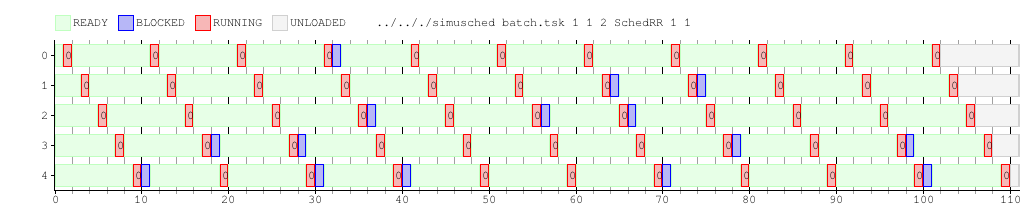
\includegraphics[width=1.1\textwidth]{img/core1q1.png}
     \caption{Round Robin con quantum 1}
\end{center}
\end{figure}

Turnarround: 105 ciclos

Waiting time: 92 ciclos 

\begin{figure}[H]
\begin{center}
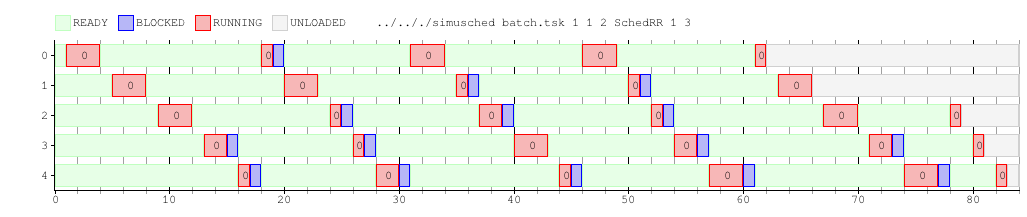
\includegraphics[width=1.1\textwidth]{img/core1q3.png}
     \caption{Round Robin con quantum 3}
\end{center}
\end{figure}

Turnarround: 74.2 ciclos

Waiting time: 60.2 ciclos 

\begin{figure}[H]
\begin{center}
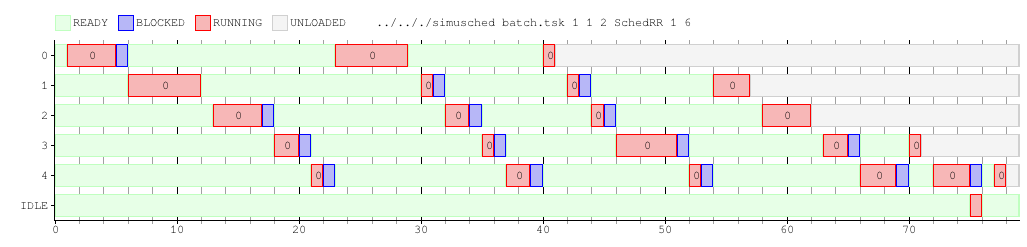
\includegraphics[width=1.1\textwidth]{img/core1q6.png}
     \caption{Round Robin con quantum 6}
\end{center}
\end{figure}

Turnarround: 62.8 ciclos

Waiting time: 47.8 ciclos 

\begin{figure}[H]
\begin{center}
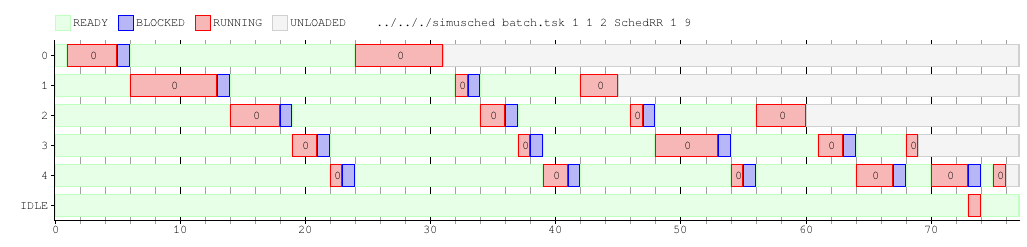
\includegraphics[width=1.1\textwidth]{img/core1q9.png}
     \caption{Round Robin con quantum 9}
\end{center}
\end{figure}

Turnarround: 56.2 ciclos

Waiting time: 42.2 ciclos 

\begin{figure}[H]
\begin{center}
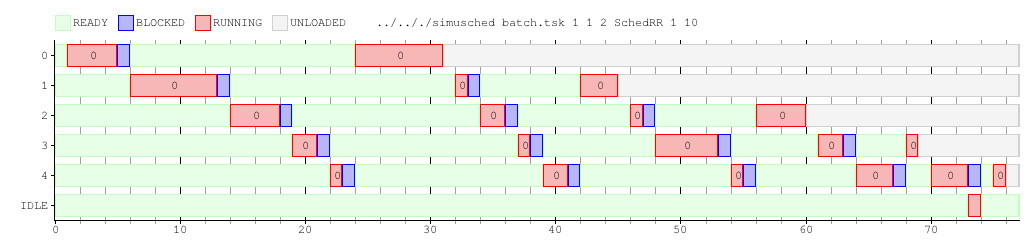
\includegraphics[width=1.1\textwidth]{img/core1q10.png}
     \caption{Round Robin con quantum 10}
\end{center}
\end{figure}

Turnarround: 56.2 ciclos

Waiting time: 42.2 ciclos 

\begin{figure}[H]
\begin{center}
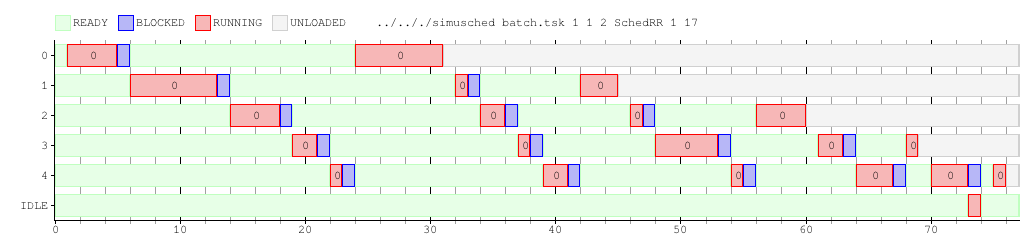
\includegraphics[width=1.1\textwidth]{img/core1q17.png}
     \caption{Round Robin con quantum 17}
\end{center}
\end{figure}

Turnarround: 56.2 ciclos

Waiting time: 42.2 ciclos

Como se puede observar ambas métricas mejoran mientras en quantum es mas alto, pero luego de tener quantum 9, las métricas dan lo mismo (por dar el mismo gráfico). Por lo tanto el valor óptimo de quantum es 9 para este tipo de test.

\subsection{Experimento con 2 cores}

\begin{figure}[H]
\begin{center}
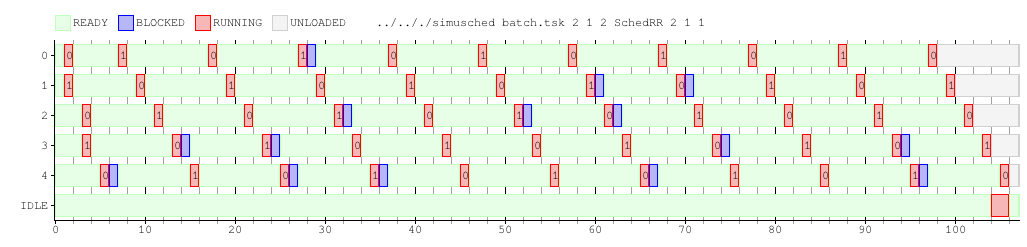
\includegraphics[width=1.1\textwidth]{img/core2q1.png}
     \caption{Round Robin con quantum 1}
\end{center}
\end{figure}

Turnarround: 102 ciclos

Waiting time: 88 ciclos 

\begin{figure}[H]
\begin{center}
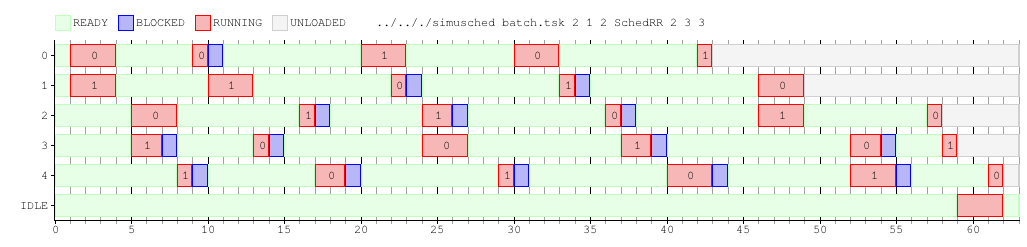
\includegraphics[width=1.1\textwidth]{img/core2q3.png}
     \caption{Round Robin con quantum 3}
\end{center}
\end{figure}

Turnarround: 54.4 ciclos

Waiting time: 40.2 ciclos 

\begin{figure}[H]
\begin{center}
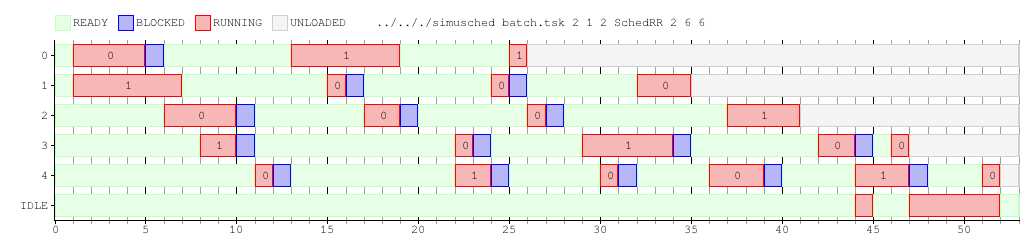
\includegraphics[width=1.1\textwidth]{img/core2q6.png}
     \caption{Round Robin con quantum 6}
\end{center}
\end{figure}

Turnarround: 40.2 ciclos

Waiting time: 26.2 ciclos 

\begin{figure}[H]
\begin{center}
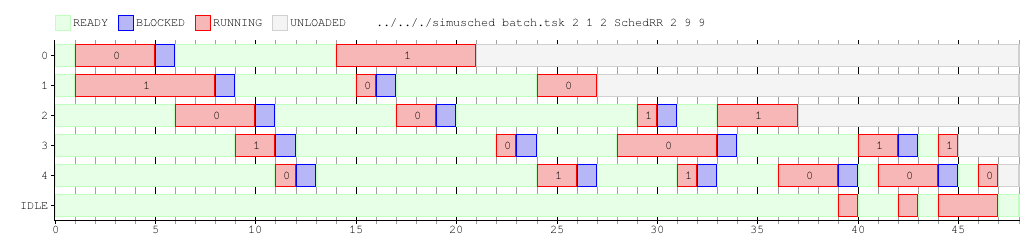
\includegraphics[width=1.1\textwidth]{img/core2q9.png}
     \caption{Round Robin con quantum 9}
\end{center}
\end{figure}

Turnarround: 35.4 ciclos

Waiting time: 21.4 ciclos 

\begin{figure}[H]
\begin{center}
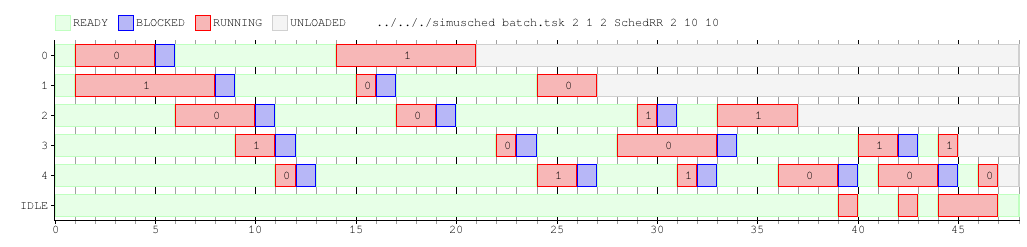
\includegraphics[width=1.1\textwidth]{img/core2q10.png}
     \caption{Round Robin con quantum 10}
\end{center}
\end{figure}

Turnarround: 35.4 ciclos

Waiting time: 21.4 ciclos 

\begin{figure}[H]
\begin{center}
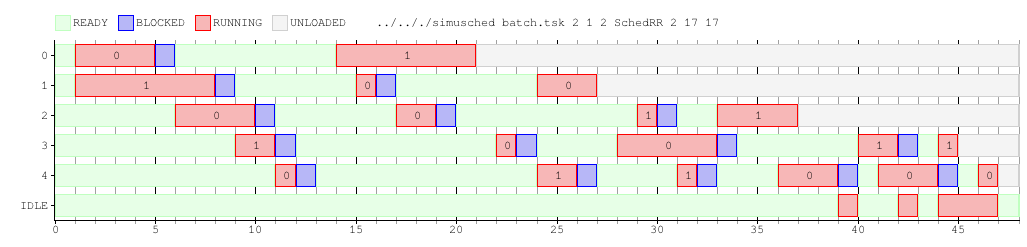
\includegraphics[width=1.1\textwidth]{img/core2q17.png}
     \caption{Round Robin con quantum 17}
\end{center}
\end{figure}

Turnarround: 56.2 ciclos

Waiting time: 42.2 ciclos

Como se puede observar ambas métricas mejoran mientras en quantum es mas alto, pero luego de tener quantum 9, las métricas dan lo mismo (por dar el mismo gráfico). Por lo tanto el valor óptimo de quantum es 9 para este tipo de test.

\subsection{Experimento con 4 cores}

\begin{figure}[H]
\begin{center}
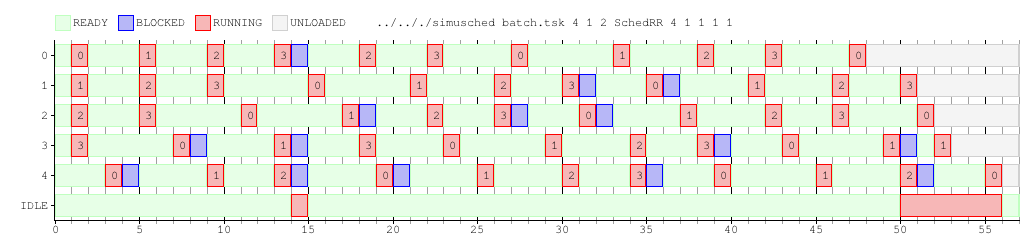
\includegraphics[width=1.1\textwidth]{img/core4q1.png}
     \caption{Round Robin con quantum 1}
\end{center}
\end{figure}

Turnarround: 51 ciclos

Waiting time: 38 ciclos 

\begin{figure}[H]
\begin{center}
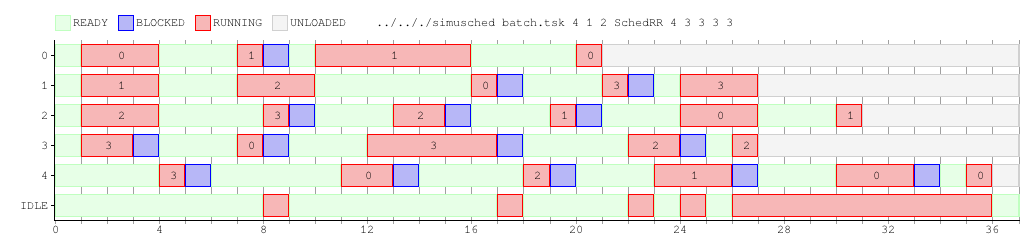
\includegraphics[width=1.1\textwidth]{img/core4q3.png}
     \caption{Round Robin con quantum 3}
\end{center}
\end{figure}

Turnarround: 28.4 ciclos

Waiting time: 14.4 ciclos 

\begin{figure}[H]
\begin{center}
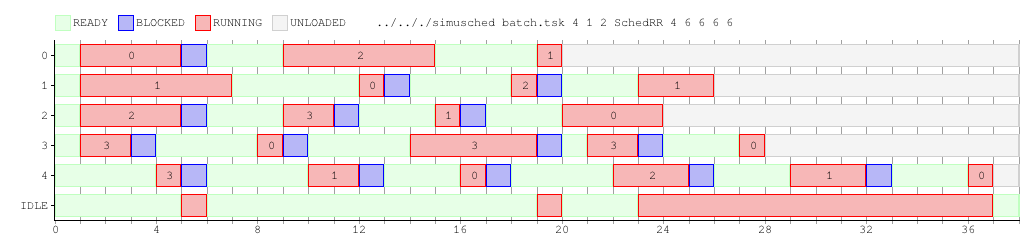
\includegraphics[width=1.1\textwidth]{img/core4q6.png}
     \caption{Round Robin con quantum 6}
\end{center}
\end{figure}

Turnarround: 27 ciclos

Waiting time: 13 ciclos 

\begin{figure}[H]
\begin{center}
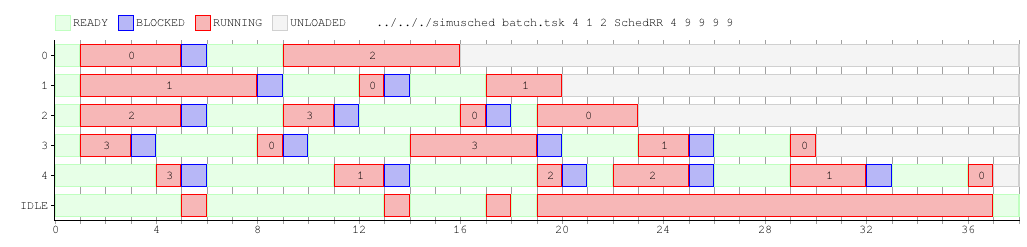
\includegraphics[width=1.1\textwidth]{img/core4q9.png}
     \caption{Round Robin con quantum 9}
\end{center}
\end{figure}

Turnarround: 25 ciclos

Waiting time: 10.2 ciclos 

\begin{figure}[H]
\begin{center}
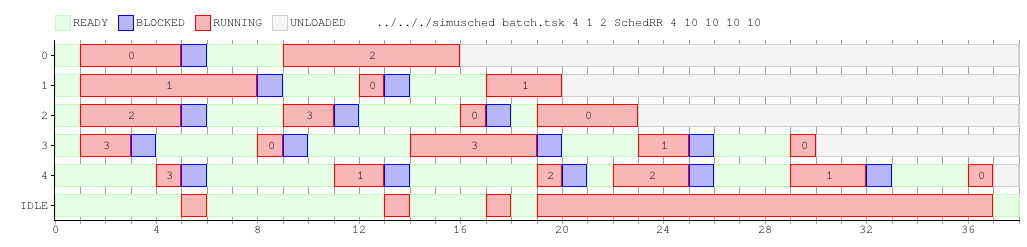
\includegraphics[width=1.1\textwidth]{img/core4q10.png}
     \caption{Round Robin con quantum 10}
\end{center}
\end{figure}

Turnarround: 25 ciclos

Waiting time: 10.2 ciclos 

\begin{figure}[H]
\begin{center}
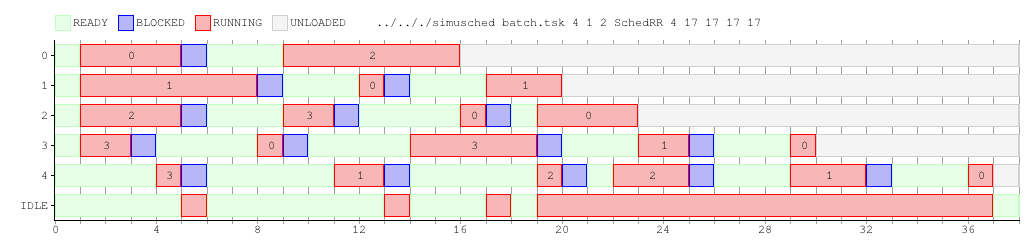
\includegraphics[width=1.1\textwidth]{img/core4q17.png}
     \caption{Round Robin con quantum 17}
\end{center}
\end{figure}

Turnarround: 56.2 ciclos

Waiting time: 42.2 ciclos

Como se puede observar ambas métricas mejoran mientras en quantum es mas alto, pero luego de tener quantum 9, las métricas dan lo mismo (por dar el mismo gráfico). Por lo tanto el valor óptimo de quantum es 9 para este tipo de test.